\documentclass{beamer}
 \usepackage{graphicx}
\usepackage[utf8]{inputenc}
 
\title{A Brief Introduction to Beamer: \\A CS251 Report by Group 02}
\author{Harshal ,  Tanmay, \quad Navneet\\140050003  140100011  140100090\\ harshal.m \quad  tanmayb \quad navneet}
\institute{IITB}
 
 
\begin{document}
 \maketitle
 \begin{frame}{Overview}
 This report is an introduction to Beamers. Beamers are very useful for making presentations and lectures and their distinct advantage over MS Powerpoint other than  being open source is customizability.
 This presentation brushes the fundamentals of beamer and how to create a title page with illustrations
 \end{frame}
 
\begin{frame}{Introduction}
\begin{enumerate}
\item<1-> Beamer is a LaTeX class to create powerful, flexible and nice-looking presentations and slides\\
\item<2-> Beamer supports syntax of other LaTeX presentation packages, including Prosper and Foils, by using compatibility packages.\\
\item<3-> Beamer provides the ability to make \"handouts\", that is a version of the output suitable for printing, without the dynamic features, so that the printed version of a slide shows the final version that will appear during the presentation. \\
\end{enumerate}
\end{frame}

\fboxsep=0pt
\noindent\fbox{%
\begin{minipage}[t]{0.48\linewidth}
\textbf{Code}\\
$\backslash$documentclass\{beamer\} \\
$\backslash$title\{Name of the title\}\\ 
$\backslash$author\{Name of the author\}\\ 
$\backslash$institute\{Name of the institute\}\\

\end{minipage}}%
\hfill
\fbox{%
\begin{minipage}[t]{0.48\linewidth}
\hfill \break
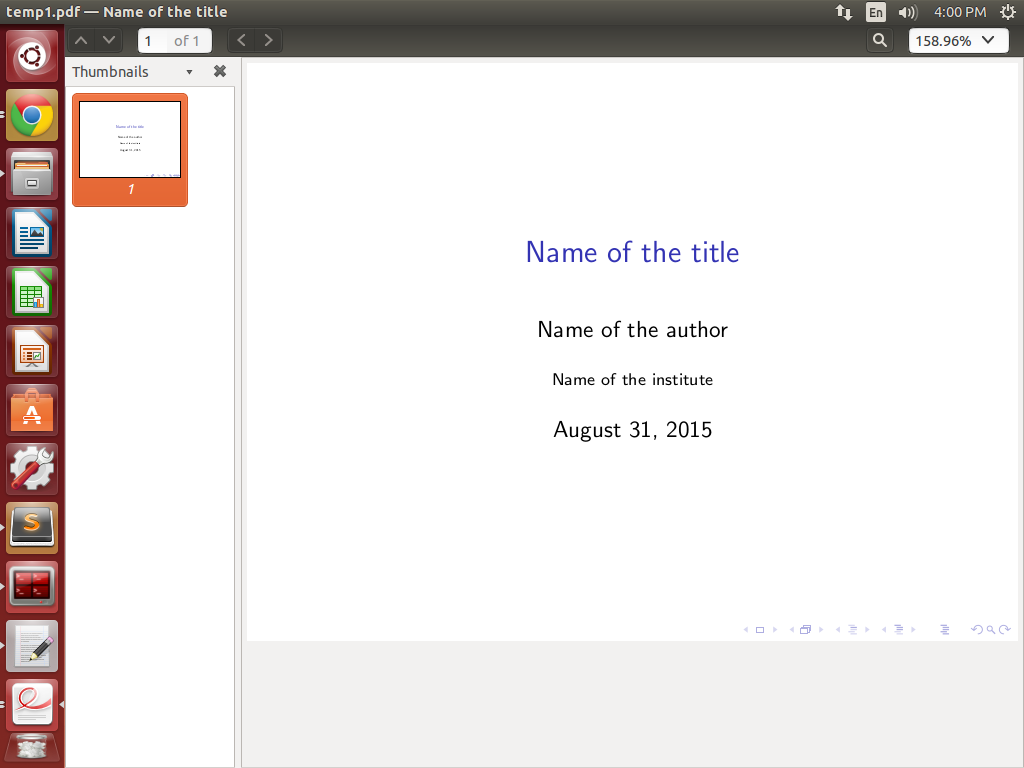
\includegraphics[width=5cm]{t}
\end{minipage}
}
\begin{frame}{Examples}
The thing I like the most about Latex othe r than its vast unicode languages is the  ability to enumerate in different ways. For eg we can change the order they appear 
\begin{enumerate}
\item<1-> Beamer is a LaTeX class to create powerful, flexible and nice-looking presentations and slides\\
\item<3-> Beamer supports syntax of other LaTeX presentation packages, including Prosper and Foils, by using compatibility packages.\\
\item<2-> Beamer provides the ability to make \"handouts\", that is a version of the output suitable for printing, without the dynamic features, so that the printed version of a slide shows the final version that will appear during the presentation. \\
\end{enumerate}
\end{frame}
\begin{frame}{Examples}
The thing I like the most about Latex othe r than its vast unicode languages is the  ability to enumerate in different ways. For eg we can change the order they appear 
\begin{enumerate}
\item<1> Beamer is a LaTeX class to create powerful, flexible and nice-looking presentations and slides\\
\item<3> Beamer supports syntax of other LaTeX presentation packages, including Prosper and Foils, by using compatibility packages.\\
\item<2> Beamer provides the ability to make \"handouts\", that is a version of the output suitable for printing, without the dynamic features, so that the printed version of a slide shows the final version that will appear during the presentation. \\
\end{enumerate}
\end{frame}

\end{document}